\definecolor{sr}{RGB}{43,131,186}
\definecolor{svi}{RGB}{215,25, 28}
\definecolor{svf}{RGB}{179,143,59}
\definecolor{g}{RGB}{0,178,93}
\definecolor{k}{RGB}{0,0,0}
\definecolor{m}{RGB}{255,0,255}

% GNUPLOT: LaTeX picture with Postscript
\begingroup
  \makeatletter
  \providecommand\color[2][]{%
    \GenericError{(gnuplot) \space\space\space\@spaces}{%
      Package color not loaded in conjunction with
      terminal option `colourtext'%
    }{See the gnuplot documentation for explanation.%
    }{Either use 'blacktext' in gnuplot or load the package
      color.sty in LaTeX.}%
    \renewcommand\color[2][]{}%
  }%
  \providecommand\includegraphics[2][]{%
    \GenericError{(gnuplot) \space\space\space\@spaces}{%
      Package graphicx or graphics not loaded%
    }{See the gnuplot documentation for explanation.%
    }{The gnuplot epslatex terminal needs graphicx.sty or graphics.sty.}%
    \renewcommand\includegraphics[2][]{}%
  }%
  \providecommand\rotatebox[2]{#2}%
  \@ifundefined{ifGPcolor}{%
    \newif\ifGPcolor
    \GPcolorfalse
  }{}%
  \@ifundefined{ifGPblacktext}{%
    \newif\ifGPblacktext
    \GPblacktexttrue
  }{}%
  % define a \g@addto@macro without @ in the name:
  \let\gplgaddtomacro\g@addto@macro
  % define empty templates for all commands taking text:
  \gdef\gplfronttext{}%
  \gdef\gplfronttext{}%
  \makeatother
  \ifGPblacktext
    % no textcolor at all
    \def\colorrgb#1{}%
    \def\colorgray#1{}%
  \else
    % gray or color?
    \ifGPcolor
      \def\colorrgb#1{\color[rgb]{#1}}%
      \def\colorgray#1{\color[gray]{#1}}%
      \expandafter\def\csname LTw\endcsname{\color{white}}%
      \expandafter\def\csname LTb\endcsname{\color{black}}%
      \expandafter\def\csname LTa\endcsname{\color{black}}%
      \expandafter\def\csname LT0\endcsname{\color[rgb]{1,0,0}}%
      \expandafter\def\csname LT1\endcsname{\color[rgb]{0,1,0}}%
      \expandafter\def\csname LT2\endcsname{\color[rgb]{0,0,1}}%
      \expandafter\def\csname LT3\endcsname{\color[rgb]{1,0,1}}%
      \expandafter\def\csname LT4\endcsname{\color[rgb]{0,1,1}}%
      \expandafter\def\csname LT5\endcsname{\color[rgb]{1,1,0}}%
      \expandafter\def\csname LT6\endcsname{\color[rgb]{0,0,0}}%
      \expandafter\def\csname LT7\endcsname{\color[rgb]{1,0.3,0}}%
      \expandafter\def\csname LT8\endcsname{\color[rgb]{0.5,0.5,0.5}}%
    \else
      % gray
      \def\colorrgb#1{\color{black}}%
      \def\colorgray#1{\color[gray]{#1}}%
      \expandafter\def\csname LTw\endcsname{\color{white}}%
      \expandafter\def\csname LTb\endcsname{\color{black}}%
      \expandafter\def\csname LTa\endcsname{\color{black}}%
      \expandafter\def\csname LT0\endcsname{\color{black}}%
      \expandafter\def\csname LT1\endcsname{\color{black}}%
      \expandafter\def\csname LT2\endcsname{\color{black}}%
      \expandafter\def\csname LT3\endcsname{\color{black}}%
      \expandafter\def\csname LT4\endcsname{\color{black}}%
      \expandafter\def\csname LT5\endcsname{\color{black}}%
      \expandafter\def\csname LT6\endcsname{\color{black}}%
      \expandafter\def\csname LT7\endcsname{\color{black}}%
      \expandafter\def\csname LT8\endcsname{\color{black}}%
    \fi
  \fi
    \setlength{\unitlength}{0.0500bp}%
    \ifx\gptboxheight\undefined%
      \newlength{\gptboxheight}%
      \newlength{\gptboxwidth}%
      \newsavebox{\gptboxtext}%
    \fi%
    \setlength{\fboxrule}{0.5pt}%
    \setlength{\fboxsep}{1pt}%
\begin{picture}(8000.00,8000.00)%
    \gplgaddtomacro\gplfronttext{%
    }%
    \gplgaddtomacro\gplfronttext{%
    }%
    \gplgaddtomacro\gplfronttext{%
      \colorrgb{0.15,0.15,0.15}%
      \put(4868,4400){\makebox(0,0)[r]{\strut{}$2^{-2}$}}%
      \colorrgb{0.15,0.15,0.15}%
      \put(4868,4680){\makebox(0,0)[r]{\strut{}$2^{-1}$}}%
      \colorrgb{0.15,0.15,0.15}%
      \put(4868,4960){\makebox(0,0)[r]{\strut{}$2^{0}$}}%
      \colorrgb{0.15,0.15,0.15}%
      \put(4868,5240){\makebox(0,0)[r]{\strut{}$2^{1}$}}%
      \colorrgb{0.15,0.15,0.15}%
      \put(4868,5520){\makebox(0,0)[r]{\strut{}$2^{2}$}}%
      \colorrgb{0.15,0.15,0.15}%
      \put(4868,5800){\makebox(0,0)[r]{\strut{}$2^{3}$}}%
      \colorrgb{0.15,0.15,0.15}%
      \put(4868,6080){\makebox(0,0)[r]{\strut{}$2^{4}$}}%
      \colorrgb{0.15,0.15,0.15}%
      \put(4868,6360){\makebox(0,0)[r]{\strut{}$2^{5}$}}%
      \colorrgb{0.15,0.15,0.15}%
      \put(4868,6640){\makebox(0,0)[r]{\strut{}$2^{6}$}}%
      \colorrgb{0.15,0.15,0.15}%
      \put(4868,6921){\makebox(0,0)[r]{\strut{}$2^{7}$}}%
      \colorrgb{0.15,0.15,0.15}%
      \put(4868,7201){\makebox(0,0)[r]{\strut{}$2^{8}$}}%
      \colorrgb{0.15,0.15,0.15}%
      \put(5095,4180){\makebox(0,0){\strut{}$1$}}%
      \colorrgb{0.15,0.15,0.15}%
      \put(6231,4180){\makebox(0,0){\strut{}$13$}}%
      \colorrgb{0.15,0.15,0.15}%
      \put(6515,4180){\makebox(0,0){\strut{}$16$}}%
      \colorrgb{0.15,0.15,0.15}%
      \put(6799,4180){\makebox(0,0){\strut{}$19$}}%
    }%
    \gplgaddtomacro\gplfronttext{%
    }%
    \gplgaddtomacro\gplfronttext{%
    }%
    \gplgaddtomacro\gplfronttext{%
    }%
    \gplgaddtomacro\gplfronttext{%
      \colorrgb{0.15,0.15,0.15}%
      \put(4868,800){\makebox(0,0)[r]{\strut{}$2^{-2}$}}%
      \colorrgb{0.15,0.15,0.15}%
      \put(4868,1080){\makebox(0,0)[r]{\strut{}$2^{-1}$}}%
      \colorrgb{0.15,0.15,0.15}%
      \put(4868,1360){\makebox(0,0)[r]{\strut{}$2^{0}$}}%
      \colorrgb{0.15,0.15,0.15}%
      \put(4868,1640){\makebox(0,0)[r]{\strut{}$2^{1}$}}%
      \colorrgb{0.15,0.15,0.15}%
      \put(4868,1920){\makebox(0,0)[r]{\strut{}$2^{2}$}}%
      \colorrgb{0.15,0.15,0.15}%
      \put(4868,2200){\makebox(0,0)[r]{\strut{}$2^{3}$}}%
      \colorrgb{0.15,0.15,0.15}%
      \put(4868,2480){\makebox(0,0)[r]{\strut{}$2^{4}$}}%
      \colorrgb{0.15,0.15,0.15}%
      \put(4868,2760){\makebox(0,0)[r]{\strut{}$2^{5}$}}%
      \colorrgb{0.15,0.15,0.15}%
      \put(4868,3040){\makebox(0,0)[r]{\strut{}$2^{6}$}}%
      \colorrgb{0.15,0.15,0.15}%
      \put(4868,3321){\makebox(0,0)[r]{\strut{}$2^{7}$}}%
      \colorrgb{0.15,0.15,0.15}%
      \put(4868,3601){\makebox(0,0)[r]{\strut{}$2^{8}$}}%
      \colorrgb{0.15,0.15,0.15}%
      \put(5078,580){\makebox(0,0){\strut{}$1$}}%
      \colorrgb{0.15,0.15,0.15}%
      \put(5548,580){\makebox(0,0){\strut{}$7$}}%
      \colorrgb{0.15,0.15,0.15}%
      \put(6173,580){\makebox(0,0){\strut{}$15$}}%
      \colorrgb{0.15,0.15,0.15}%
      \put(6799,580){\makebox(0,0){\strut{}$23$}}%
    }%
    \gplgaddtomacro\gplfronttext{%
      \colorrgb{0.15,0.15,0.15}%
      \put(5400,7619){\makebox(0,0){\strut{}{\color{k}{\rule[0.6mm]{0.5cm}{0.5mm}}} $\dfrac{|\theta-\hat{\theta}[k]|}{\gamma}$}}%
      \put(6700,7619){\makebox(0,0){\strut{}{\color{g}{\rule[0.6mm]{0.5cm}{0.5mm}}} $2^{-1}$}}%
      \put(1000,7519){\makebox(0,0){\strut{}{\color{k}{\rule[0.6mm]{0.5cm}{0.5mm}}} $\bm{M}$}}%
      \put(1750,7519){\makebox(0,0){\strut{}{\color{sr}{\rule[0.6mm]{0.5cm}{0.5mm}}} $\bm{p}$}}%
      \put(2500,7519){\makebox(0,0){\strut{}{\color{svi}{\rule[0.6mm]{0.5cm}{0.5mm}}} $\hat{\bm{p}}[0]$}}%
      \put(3500,7519){\makebox(0,0){\strut{}{\color{svf}{\rule[0.6mm]{0.5cm}{0.5mm}}} $\hat{\bm{p}}[k_{\max}]$}}%

      \put(5100,3869){\makebox(0,0){\strut{}$\nu$}}%
      \put(5400,3869){\makebox(0,0){\strut{}\fcolorbox{black}{sinisn0}{\rule{0pt}{6pt}\rule{6pt}{0pt} 0}}} %
      \put(5800,3869){\makebox(0,0){\strut{}\fcolorbox{black}{sinisn1}{\rule{0pt}{6pt}\rule{6pt}{0pt} 1}}} %
      \put(6200,3869){\makebox(0,0){\strut{}\fcolorbox{black}{sinisn2}{\rule{0pt}{6pt}\rule{6pt}{0pt} 2}}} %
      \put(6600,3869){\makebox(0,0){\strut{}\fcolorbox{black}{sinisn3}{\rule{0pt}{6pt}\rule{6pt}{0pt} 3}}} %

      \put(2300,4039){\makebox(0,0){\strut{} Fourier-Mellin}}%
      \put(2300,250){\makebox(0,0){\strut{} Προκρούστης}}%

      \put(5899,250){\makebox(0,0){\strut{}Αριθμός επαναλήψεων $k$}}%
    }
    \put(0,0){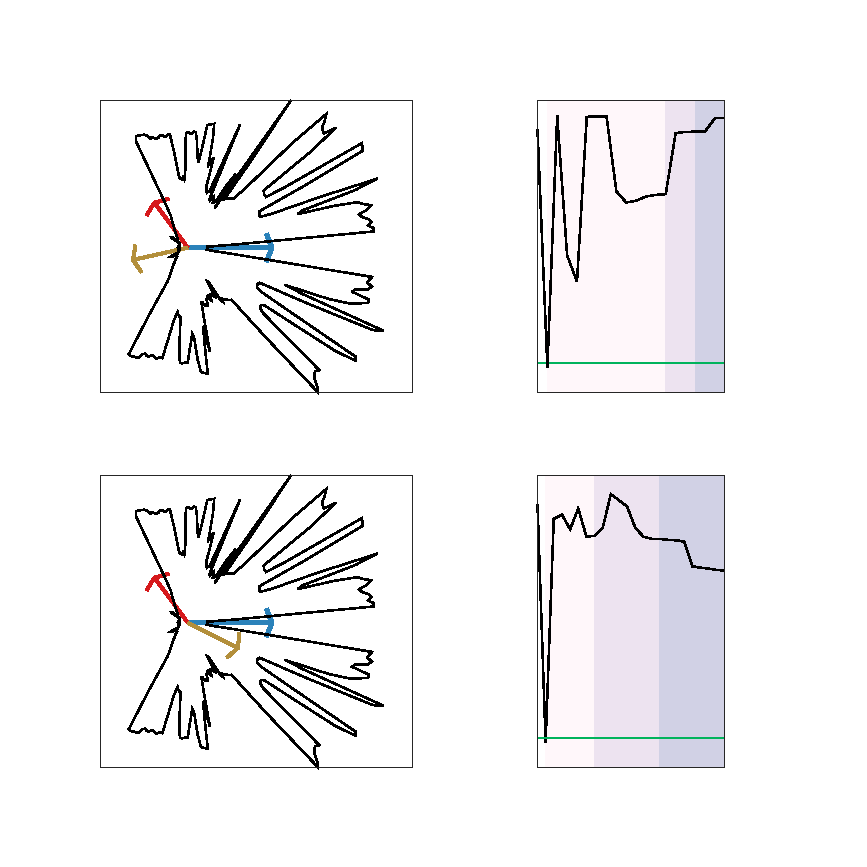
\includegraphics{./figures/parts/02/chapters/04/sections/02/sinis}}%
    \gplfronttext
  \end{picture}%
\endgroup
